%\documentclass[12pt]{article}

\questionheader{ex:s2.10}


%%%%%%%%%%%%%%%%%%
\subsection*{\Conceptual}
%%%%%%%%%%%%%%%%%%

%%%%%%%%%%%%%%%%%%%%%%%%%%%%%%%%
\begin{question}[M200 2010A] %4
\begin{enumerate}[(a)]
\item
Does the function $f(x, y) = x^2 +y^2$ have a maximum or a minimum on the curve $xy = 1$?
Explain.
\item
Find all maxima and minima of $f(x, y)$ on the curve $xy = 1$.
\end{enumerate}
\end{question}

%\begin{hint}
%
%\end{hint}

\begin{answer}
(a) $f$ does not have a maximum. It does have a minimum.

(b) The minima are at $\pm (1,1)$, where $f$ takes the value $2$.
\end{answer}
\begin{solution}
(a) 
$f(x, y) = x^2 +y^2$ is the square of the distance from the point $(x,y)$
to the origin. There are points on the curve $xy=1$ that have either $x$ or
$y$ arbitrarily large and so whose distance from the origin is arbitrarily
large. So $f$ has no maximum on the curve. On the other hand $f$ will have 
a minimum, achieved at the points of $xy=1$ that are closest to the origin.

(b) On the curve $xy=1$ we have $y=\frac{1}{x}$ and hence
$f=x^2+\frac{1}{x^2}$. As
\begin{align*}
\diff{}{x}\left(x^2+\frac{1}{x^2}\right)
=2x-\frac{2}{x^3}
=\frac{2}{x^3}(x^4-1)
\end{align*}
and as no point of the curve has $x=0$, the minimum is achieved when $x=\pm 1$. So the minima are at $\pm (1,1)$, where $f$ takes the value $2$.
\end{solution}

%%%%%%%%%%%%%%%%%%%%%%%%%%%%%%%%
\begin{question}
The surface $S$ is given by the equation $g(x,y,z)=0$.
You are walking on $S$ measuring the function $f(x,y,z)$ as you go. 
You are currently at the point $(x_0,y_0,z_0)$ where $f$ takes its 
largest value on $S$, and are walking in the direction $\vd\ne\vZero$. Because 
you are walking on $S$, the vector $\vd$ is tangent to $S$ at $(x_0,y_0,z_0)$. 
\begin{enumerate}[(a)]
\item
What is the directional derivative of $f$ at $(x_0,y_0,z_0)$ in 
the direction $\vd$? Do not use the method of Lagrange multipliers.
\item
What is the directional derivative of $f$ at $(x_0,y_0,z_0)$ in 
the direction $\vd$? This time use the method of Lagrange multipliers.
\end{enumerate}
\end{question}

\begin{hint}
(a) The function $f$ decreases, or at least does not increase, as you leave 
$(x_0,y_0,z_0)$ in the direction $\vd$.  
The function $f$ also decreases, or at least does not increase, as you leave 
$(x_0,y_0,z_0)$ in the direction $-\vd$.
\end{hint}

\begin{answer}
(a), (b) $0$
\end{answer}

\begin{solution}
(a) As you leave $(x_0,y_0,z_0)$ walking in the direction $\vd\ne\vZero$,
$f$ has to be decreasing, or at  least not increasing, because $f$ takes 
its largest value on $S$ at $(x_0,y_0,z_0)$. So the directional derivative
\begin{equation*}
D_{\vd/|\vd|}f(x_0,y_0,z_0)=\vnabla f(x_0,y_0,z_0)\cdot\frac{\vd}{|\vd|}\le 0
\tag{E1}\end{equation*}
As you leave $(x_0,y_0,z_0)$ walking in the direction $-\vd\ne\vZero$,
$f$ also has to be decreasing, or at  least not increasing, because $f$ 
still takes its largest value on $S$ at $(x_0,y_0,z_0)$. So the 
directional derivative
\begin{equation*}
D_{-\vd/|\vd|}f(x_0,y_0,z_0)=-\vnabla f(x_0,y_0,z_0)\cdot\frac{\vd}{|\vd|}\le 0
\tag{E2}\end{equation*}
(E1) and (E2) can both be true only if the directional derivative
\begin{equation*}
D_{\vd/|\vd|}f(x_0,y_0,z_0)=\vnabla f(x_0,y_0,z_0)\cdot\frac{\vd}{|\vd|} = 0
\end{equation*}

(b) By Definition \eref{CLP200}{def dri deriv} in the CLP-3 text, the 
directional derivative is
\begin{equation*}
D_{\vd/|\vd|}f(x_0,y_0,z_0)=\vnabla f(x_0,y_0,z_0)\cdot\frac{\vd}{|\vd|}
\end{equation*}
\begin{itemize}
\item
As $(x_0,y_0,z_0)$ is a local maximum for $f$ on $S$, the method of
Lagrange multipliers, Theorem \eref{CLP200}{thm Lagrange} in the CLP-3 text, 
gives that $\vnabla f(x_0,y_0,z_0) =\la\vnabla g(x_0,y_0,z_0)$ for some $\la$.
\item
By Theorem \eref{CLP200}{thm tan plane G}, the vector $\vnabla g(x_0,y_0,z_0)$
is perpendicular to the surface $S$ at $(x_0,y_0,z_0)$, and, in particular,
is perpendicular to the vector $\vd$, which after all is tangent to the surface 
$S$ at $(x_0,y_0,z_0)$. 
\end{itemize}
So $\vnabla g(x_0,y_0,z_0)\cdot\vd=0$ and the directional derivative
\begin{equation*}
D_{\vd/|\vd|}f(x_0,y_0,z_0)=\vnabla f(x_0,y_0,z_0)\cdot\frac{\vd}{|\vd|}=0
\end{equation*}
\end{solution}





%%%%%%%%%%%%%%%%%%
\subsection*{\Procedural}
%%%%%%%%%%%%%%%%%%


%%%%%%%%%%%%%%%%%%%%%%%%%%%%%%%%
\begin{question}
Find the maximum and minimum values of the function  
$f(x,y,z)=x+y-z$ on the sphere $x^2+y^2+z^2=1$.
\end{question}

%\begin{hint}
%
%\end{hint}

\begin{answer}
The max is $f=\sqrt{3}$ and the min is $f=-\sqrt{3}$.
\end{answer}

\begin{solution}
We are to find the maximum and minimum of $f(x,y,z)=x+y-z$
subject to the constraint $g(x,y,z) = x^2+y^2+z^2 -1=0$.
According to the method of Lagrange multipliers, we need to find 
all solutions to
\begin{alignat*}{7}
f_x = 1 = 2\la x  &= \la g_x 
      \quad&&\implies\quad && x=\frac{1}{2\la} \tag{E1} \\ 
f_y = 1 = 2\la y &= \la g_y 
      \quad&&\implies\quad && y=\frac{1}{2\la}\tag{E2} \\ 
f_z = -1 = 2\la z &= \la g_z 
       \quad&&\implies\quad && z=-\frac{1}{2\la} \tag{E3} \\ 
x^2+y^2+z^2&=1 
       \quad&&\implies\quad &&3\left(\frac{1}{2\la}\right)^2=1
\quad&&\implies\quad & \la&=\pm\frac{\sqrt{3}}{2}\tag{E4}
\end{alignat*}
Thus the critical points are 
$\big(-\frac{1}{\sqrt{3}},-\frac{1}{\sqrt{3}},\frac{1}{\sqrt{3}}\big)$,
where $f=-\sqrt{3}$
and 
$\big(\frac{1}{\sqrt{3}},\frac{1}{\sqrt{3}},-\frac{1}{\sqrt{3}}\big)$,
where $f=\sqrt{3}$. So, the max is $f=\sqrt{3}$ and the min is 
$f=-\sqrt{3}$.
\end{solution}

%%%%%%%%%%%%%%%%%%%%%%%%%%%%%%%%
\begin{question}
Find $a,\ b$ and $c$ so that the volume $\frac{4\pi}{3} abc$ of an ellipsoid
$\frac{x^2}{a^2}+\frac{y^2}{b^2}+\frac{z^2}{c^2}=1$ passing through
the point $(1,2,1)$ is as small as possible.
\end{question}

\begin{hint}
The ellipsoid $\frac{x^2}{a^2}+\frac{y^2}{b^2}+\frac{z^2}{c^2}=1$ passes 
through the point $(1,2,1)$ if and only if 
$\frac{1}{a^2}+\frac{4}{b^2}+\frac{1}{c^2}=1$.
\end{hint}

\begin{answer}
$a=c=\sqrt{3},\ b=2\sqrt{3}$.
\end{answer}

\begin{solution}
The ellipsoid $\frac{x^2}{a^2}+\frac{y^2}{b^2}+\frac{z^2}{c^2}=1$ passes 
through the point $(1,2,1)$ if and only if 
$\frac{1}{a^2}+\frac{4}{b^2}+\frac{1}{c^2}=1$.
We are to minimize  $f(a,b,c)=\frac{4}{3}\pi abc$ subject to the constraint 
that $g(a,b,c) = \frac{1}{a^2}+\frac{4}{b^2}+\frac{1}{c^2} -1=0$.
According to the method of Lagrange multipliers, we need to find 
all solutions to
\begin{alignat*}{7}
f_a = \frac{4}{3}\pi bc = -\frac{2\la}{a^3}  &= \la g_a 
      \quad&&\implies\quad && \frac{3}{2\pi}\la=-a^3bc \tag{E1} \\ 
f_b = \frac{4}{3}\pi ac = - \frac{8\la}{b^3} &= \la g_b 
      \quad&&\implies\quad && \frac{3}{2\pi}\la=-\frac{1}{4}ab^3c \tag{E2} \\ 
f_c = \frac{4}{3}\pi ab = -\frac{2\la}{c^3} &= \la g_c 
       \quad&&\implies\quad && \frac{3}{2\pi}\la=-abc^3 \tag{E3} \\ 
\frac{1}{a^2}+\frac{4}{b^2}+\frac{1}{c^2}&=1 \tag{E4}
\end{alignat*}
The equations $-\frac{3}{2\pi}\la=a^3bc=\frac{1}{4}ab^3c$ force $b=2a$
(since we want $a,b,c>0$). The equations $-\frac{3}{2\pi}\la=a^3bc=abc^3$ force 
$a=c$. Hence, by (E4), 
\begin{align*}
1=\frac{1}{a^2}+\frac{4}{b^2}+\frac{1}{c^2}=\frac{3}{a^2}
\implies a=c=\sqrt{3},\ b=2\sqrt{3}
\end{align*}
\end{solution}


%%%%%%%%%%%%%%%%%%%%%%%%%%%%%%%%
\begin{question}[M200 2005D] %6
Use the Method of Lagrange Multipliers to find the minimum value of 
$z = x^2 + y^2$ subject to $x^2 y = 1$. At which point or points
does the minimum occur?
\end{question}

%\begin{hint}
%
%\end{hint}

\begin{answer}
The minimum value is 
$2^{\frac{1}{3}} + 2^{-\frac{2}{3}}
       =\frac{3}{2}\root{3}\of{2}
       =\frac{3}{\sqrt[3]{4}}$ at
$\big(\pm 2^{\frac{1}{6}}\,,\, 2^{-\frac{1}{3}}\big)$.
\end{answer}

\begin{solution}
So we are to minimize  $f(x,y) = x^2+y^2 $
subject to the constraint $g(x,y) = x^2 y -1=0$.
According to the method of Lagrange multipliers, we need to find 
all solutions to
\begin{align*}
f_x = 2x &=2 \la xy = \la g_x \tag{E1} \\ 
f_y = 2y &= \la x^2 = \la g_y \tag{E2} \\ 
x^2y&=1 \tag{E3}
\end{align*}
\begin{itemize}
\item
Equation (E1), $2x(1-\la y)=0$, gives that either $x=0$ or $\la y=1$. 
\item
But substituting $x=0$ in (E3) gives $0=1$, which is impossible.
\item
Also note that $\la=0$ is impossible, since substituting $\la=0$ in (E1)
and (E2) gives $x=y=0$, which violates (E3).
\item
So $y=\frac{1}{\la}$. 
\item
Substituting $y=\frac{1}{\la}$ into (E2) gives $\frac{2}{\la} = \la x^2$
or $x^2=\frac{2}{\la^2}$. So $x=\pm\frac{\sqrt{2}}{\la}$.
\item
Substituting $y=\frac{1}{\la}$, $x=\pm\frac{\sqrt{2}}{\la}$ into (E3) gives
$\frac{2}{\la^3} =1$ or $\la^3 =  2$ or
$\la= \root{3}\of{2}$.
\item
$\la= 2^{1/3}$ gives $x=\pm 2^{\frac{1}{2}-\frac{1}{3}}=\pm 2^{\frac{1}{6}}$
   and $y= 2^{-\frac{1}{3}}$.
\end{itemize}
So the two critical points are $\big(2^{\frac{1}{6}}\,,\,2^{-\frac{1}{3}}\big)$
and $\big(-2^{\frac{1}{6}}\,,\,2^{-\frac{1}{3}}\big)$. For both of these
critical points, 
\begin{equation*}
x^2+y^2= 2^{\frac{1}{3}} + 2^{-\frac{2}{3}}
       = 2^{\frac{1}{3}} + \frac{1}{2}2^{\frac{1}{3}} 
       =\frac{3}{2}\root{3}\of{2}
       =\frac{3}{\sqrt[3]{4}}
\end{equation*}
\end{solution}

%%%%%%%%%%%%%%%%%%%%%%%%%%%%%%%%
\begin{question}[M200 2006A] %4
Use the Method of Lagrange Multipliers to find the radius of the base 
and the height of a right circular cylinder of maximum volume which can 
be fit inside the unit sphere $x^2 + y^2 + z^2 = 1$.
\end{question}

%\begin{hint}
%
%\end{hint}

\begin{answer}
$\text{radius}=\sqrt{\frac{2}{3}}$
and $\text{height}=\frac{2}{\sqrt{3}}$.
\end{answer}

\begin{solution}
 Let $r$ and $h$ denote the radius and height, respectively, of the cylinder. We can always choose our coordinate system so that the axis of
the cylinder is parallel to the $z$--axis.  
\begin{itemize}
\item
If the axis of the cylinder does
not lie exactly on the $z$--axis, we can enlarge the cylinder sideways.
(See the figure on the left below. It shows the $y=0$ cross--section of
the cylinder.) So we can assume that the axis of the cylinder lies on the $z$--axis  
\item
If the top and/or the bottom of the cylinder does not touch the sphere
$x^2+y^2+z^2=1$, we can enlarge the cylinder vertically. (See the
central figure below.) 
\item
So we may assume that the cylinder is
\begin{equation*}
\Set{(x,y,z)}{x^2+y^2\le r^2,\ -h/2\le z\le h/2}
\end{equation*}
with $r^2+(h/2)^2=1$. See the figure on the right below.
\end{itemize}

\begin{center}
     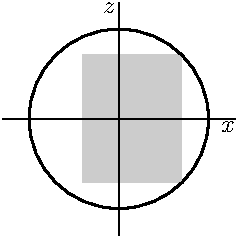
\includegraphics{OE06A_4r.pdf}\quad
     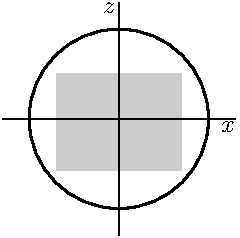
\includegraphics{OE06A_4h.pdf}
     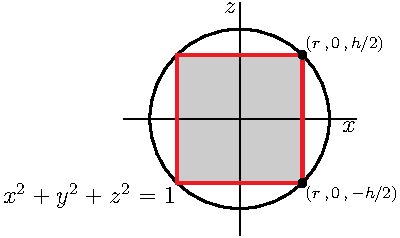
\includegraphics{OE06A_4.pdf}
\end{center}

So we are to maximize the volume, $f(r,h) = \pi r^2 h$, of the cylinder
subject to the constraint $g(r,h) = r^2+ \frac{h^2}{4} -1=0$.
According to the method of Lagrange multipliers, we need to find 
all solutions to
\begin{align*}
f_r = 2\pi r h &=2 \la r = \la g_r \tag{E1} \\ 
f_h = \pi r^2 &= \la \frac{h}{2} = \la g_h \tag{E2} \\ 
r^2+ \frac{h^2}{4}&=1 \tag{E3}
\end{align*}
Equation (E1), $2r(\pi h-\la)=0$, gives that either $r=0$ or $\la=\pi h$. 
Clearly $r=0$ cannot give the maximum volume, so $\la=\pi h$.
Substituting $\la=\pi h$ into (E2) gives
\begin{equation*}
\pi r^2 = \frac{1}{2}\pi h^2
\implies r^2=\frac{h^2}{2}
\end{equation*}
Substituting $r^2=\frac{h^2}{2}$ into (E3) gives
\begin{align*}
\frac{h^2}{2} + \frac{h^2}{4} =1
\implies h^2 =\frac{4}{3}
\end{align*}
Clearly both $r$ and $h$ have to be positive, so $h=\frac{2}{\sqrt{3}}$
and $r=\sqrt{\frac{2}{3}}$.
\end{solution}


%%%%%%%%%%%%%%%%%%%%%%%%%%%%%%%%
\begin{question}[M200 2006D] %3b
Use the method of Lagrange Multipliers to find the maximum
and minimum values of
\begin{equation*}
f(x, y) = xy
\end{equation*}
subject to the constraint
\begin{equation*}
x^2 + 2y^2 = 1.
\end{equation*}
\end{question}

%\begin{hint}
%
%\end{hint}

\begin{answer}
The maximum and minimum values of $f$ are $\frac{1}{2\sqrt{2}}$
and $-\frac{1}{2\sqrt{2}}$, respectively.
\end{answer}

\begin{solution}
For this problem the objective function is $f(x,y) = xy$
and the constraint function is $g(x,y)=x^2 + 2y^2 - 1$. 
To apply the method of Lagrange multipliers we need $\vnabla f$
and $\vnabla g$. So we start by computing the first order derivatives
of these functions.
\begin{equation*}
f_x=y\qquad
f_y=x\qquad
g_x=2x\qquad
g_y=4y
\end{equation*}
So, according to the method of Lagrange multipliers, we need to find all solutions to
\begin{align*}
y&=\la (2x) \tag{E1}\\
x&=\la (4y)  \tag{E2}\\
x^2+2y^2-1&=0 \tag{E3}
\end{align*}
First observe that none of $x$, $y$, $\la$ can be zero, because if at
least one of them is zero, then (E1) and (E2) force $x=y=0$, which violates
(E3). Dividing (E1) by (E2) gives $\frac{y}{x} = \frac{x}{2y}$
so that $x^2=2y^2$ or $x=\pm \sqrt{2}\,y$. Then (E3) gives
\begin{align*}
2y^2+2y^2=1
\iff y=\pm\frac{1}{2}
\end{align*}
The method of Lagrange multipliers, Theorem \eref{CLP200}{thm Lagrange}
in the CLP-3 text, gives
that the only possible locations of the maximum and minimum of the function
$f$ are $\left(\pm\frac{1}{\sqrt{2}},\pm\frac{1}{2}\right)$. 
So the maximum and minimum values of $f$ are $\frac{1}{2\sqrt{2}}$
and $-\frac{1}{2\sqrt{2}}$, respectively.
\end{solution}

%%%%%%%%%%%%%%%%%%%%%%%%%%%%%%%%
\begin{question}[M200 2008A] %5
Find the maximum and minimum values of $f(x,y) = x^2 + y^2$ 
subject to the constraint $x^4 + y^4 = 1$.
\end{question}

%\begin{hint}
%
%\end{hint}

\begin{answer}
min$=1$, max$=\sqrt{2}$.
\end{answer}

\begin{solution}
This is a constrained optimization problem with the objective function being
$f(x,y) = x^2 + y^2$ and the constraint function being
$g(x,y) =x^4 + y^4 - 1$.
By Theorem \eref{CLP200}{thm Lagrange} in the CLP-3 text, any minimum
or maximum $(x,y)$ must obey the  Lagrange multiplier equations
\begin{align*}
f_x = 2x &=4 \la x^3 = \la g_x \tag{E1} \\ 
f_y = 2y &=4 \la y^3 = \la g_y \tag{E2} \\ 
x^4 + y^4 &= 1 \tag{E3}
\end{align*}
for some real number $\la$. By equation (E1), $2x(1-2\la x^2)=0$, which is
obeyed if and only if at least one of $x=0$, $2\la x^2=1$ is obeyed.
Similarly, by equation (E2), $2y(1-2\la y^2)=0$, which is
obeyed if and only if at least one of $y=0$, $2\la y^2=1$ is obeyed.
\begin{itemize}
\item 
If $x=0$, (E3) reduces to $y^4=1$ or $y=\pm 1$. At both
$\big(0,\pm 1\big)$ we have $f\big(0,\pm1\big)=1$.
\item 
If $y=0$, (E3) reduces to $x^4=1$ or $x=\pm 1$. At both
$\big(\pm 1,0\big)$ we have $f\big(\pm1,0\big)=1$.
\item
If both $x$ and $y$ are nonzero, we have $x^2=\frac{1}{2\lambda}=y^2$.
Then (E3) reduces to
\begin{align*}
2x^4=1 
\end{align*}
so that
$x^2=y^2=\frac{1}{\sqrt{2}}$ and $x=\pm 2^{-1/4}$,
$y=\pm 2^{-1/4}$.  At all four of these points, we
have $f=\sqrt{2}$.

\end{itemize}
So the minimum value of $f$ on $x^4+y^4=1$ is $1$ and
the maximum value of $f$ on $x^4+y^4=1$ is $\sqrt{2}$.  
\end{solution}

%%%%%%%%%%%%%%%%%%%%%%%%%%%%%%%%
\begin{question}[M200 2008D] %5b
Use Lagrange multipliers to find the points on the sphere
$z^2 + x^2 + y^2 - 2y - 10 = 0$ closest to and farthest from the point 
$(1, -2, 1)$.
\end{question}

%\begin{hint}
%
%\end{hint}

\begin{answer}
$(1,-2,1)$  is the closest point. 
$(-1,4,-1)$ is the farthest point.
\end{answer}

\begin{solution}
The function $f(x,y,z)=(x-1)^2+(y+2)^2+(z-1)^2$ gives the square of 
the distance from  the point $(x,y,z)$ to the point $(1,-2,1)$. 
So it suffices to find the $(x,y,z)$ which minimizes $
f(x,y,z)=(x-1)^2+(y+2)^2+(z-1)^2$ subject 
to the constraint $g(x,y,z) = z^2 + x^2 + y^2 - 2y - 10=0$.
By Theorem \eref{CLP200}{thm Lagrange} in the CLP-3 text, any local minimum
or maximum $(x,y,z)$ must obey the  Lagrange multiplier equations
\begin{align*}
f_x = 2(x-1) &= 2 \la x = \la g_x \tag{E1} \\ 
f_y = 2(y+2) &=2 \la (y-1)  = \la g_y \tag{E2} \\ 
f_z = 2(z-1) &= 2\la z = \la g_z \tag{E3} \\ 
z^2 + x^2 + y^2 - 2y &= 10 \tag{E4}
\end{align*}
for some real number $\la$. Now
\begin{align*}
\text{(E1)} &\implies x=\frac{1}{1-\la} \\
\text{(E2)} &\implies y=-\frac{2+\la}{1-\la} \\
\text{(E3)} &\implies z=\frac{1}{1-\la} 
\end{align*}
(Note that $\la$ cannot be $1$, because if it were (E1) would reduce to $-2=0$.)
Substituting these into (E4), and using that 
\begin{equation*}
y-2=-\frac{2+\la}{1-\la} -\frac{2-2\la}{1-\la}=-\frac{4-\la}{1-\la}
\end{equation*}
gives
\begin{align*}
&\frac{1}{{(1-\la)}^2}+\frac{1}{{(1-\la)}^2} 
   +\frac{2+\la}{1-\la}\ \frac{4-\la}{1-\la} = 10 \\
\iff & 2+(2+\la)(4-\la) = 10 (1-\la)^2 \\
\iff & 11\la^2 -22\la =0 \\
\iff & \la=0\text{ or }\la=2
\end{align*}
When $\la=0$, we have $(x,y,z) = (1,-2,1)$ (nasty!), which gives 
distance zero and so is certainly the closest point. 
When $\la=2$, we have $(x,y,z) = (-1,4,-1)$, which does not give 
distance zero and so is certainly the farthest point.

\end{solution}

%%%%%%%%%%%%%%%%%%%%%%%%%%%%%%%%
\begin{question}[M200 2009A] %4
Use Lagrange multipliers to find the maximum and minimum values of the 
function $f(x,y,z) = x^2 + y^2 -\frac{1}{20} z^2$ on the curve of 
intersection of the plane $x + 2y + z = 10$ and the paraboloid 
$x^2 + y^2 - z = 0$.
\end{question}

%\begin{hint}
%
%\end{hint}

\begin{answer}
The maximum is $5$ and the minimum is $0$.
\end{answer}

\begin{solution}
We are to maximize and minimize $f(x,y,z)=x^2 + y^2 -\frac{1}{20} z^2$ 
subject to the constraints $g(x,y,z)=x + 2y + z - 10=0$ and 
$h(x,y,z) = x^2 + y^2 - z=0$.
By Theorem \eref{CLP200}{thm doubleLagrange} in the CLP-3 text, 
any local minimum or maximum $(x,y,z)$ must obey the  double Lagrange 
multiplier equations
\begin{align*}
f_x = 2x &=\la + 2 \mu x = \la g_x +\mu h_x\tag{E1} \\ 
f_y = 2y &=2\la + 2 \mu y = \la g_y +\mu h_y\tag{E2} \\ 
f_z = -\frac{z}{10} &=\la - \mu  = \la g_z +\mu h_z\tag{E3} \\ 
x + 2y + z &= 10\tag{E4} \\
x^2 + y^2 - z &= 0 \tag{E5}
\end{align*}
for some real numbers $\la$ and $\mu$.

Equation (E1) gives $2(1-\mu)x=\la$ and equation (E2) gives
$(1-\mu)y=\la$. So
\begin{align*}
2(1-\mu)x=(1-\mu)y
\implies 
(1-\mu)(2x-y)=0
\end{align*}
So at least one of $\mu=1$ and $y=2x$ must be true.
\begin{itemize}
\item 
If $\mu=1$, equations (E1) and (E2) both reduce to $\la=0$
and then the remaining equations reduce to
\begin{align*}
-\frac{z}{10} &=-1\tag{E3} \\ 
x + 2y + z &= 10\tag{E4} \\
x^2 + y^2 - z &= 0 \tag{E5}
\end{align*}
Then (E3) implies $z=10$, and (E4) in turn implies $x+2y+10=10$ so
that $x=-2y$. Finally, substituting $z=10$ and $x=-2y$ into (E5) gives 
\begin{align*}
4y^2+y^2-10=0
\iff 5y^2=10
\iff y=\pm\sqrt{2}
\end{align*}


\item If $y=2x$, equations (E4) and (E5) reduce to
\begin{align*}
5x + z &= 10\tag{E4} \\
5x^2  - z &= 0 \tag{E5}
\end{align*}
Substituting $z=5x^2$, from (E5), into (E4) gives
\begin{align*}
5x^2+5x-10=0
\iff 
x^2+x-2=0
\iff
(x+2)(x-1)=0
\end{align*}
So we have either $x=-2$, $y=2x=-4$, $z=5x^2=20$
               or $x=1$, $y=2x=2$, $z=5x^2=5$. 
(In both cases, we could now solve (E1) and (E3) for $\la$ and $\mu$,
but we don't care what the values of $\la$ and $\mu$ are.) 

\end{itemize}
So we have the following candidates for the locations of the min and max
\begin{center}
\renewcommand{\arraystretch}{1.3}
     \begin{tabular}{|c|c|c|c|c|}
     \hline
       point
       &$(-2\sqrt{2},\sqrt{2}, 10)$
       &$(2\sqrt{2},-\sqrt{2}, 10)$
       &$(-2,-4,20) $
       &$(1,2,5) $ \\ \hline
       value of $f$
       &$8+2-5$
       &$8+2-5$
       &$4+16-20$
       &$1+4-\frac{25}{20}$\\ \hline
       &max
       &max 
       &min 
       & \\ \hline
     \end{tabular}
\renewcommand{\arraystretch}{1.0}
\end{center}
So the maximum is $5$ and the minimum is $0$.
\end{solution}

%%%%%%%%%%%%%%%%%%%%%%%%%%%%%%%%
\begin{question}[M200 2010D] %4b
Find the point $P = (x, y, z)$ (with $x$, $y$ and $z> 0$) on the surface $x^3 y^2 z = 6 \sqrt{3}$
that is closest to the origin.
\end{question}

%\begin{hint}
%
%\end{hint}

\begin{answer}
$\big(\sqrt{3}\,,\,\sqrt{2}\,,\,1\big)$
\end{answer}

\begin{solution}
The function $f(x,y,z)=x^2+y^2+z^2$ gives the square of the distance from 
the point $(x,y,z)$ to the origin. So it suffices to find the $(x,y,z)$
(in the first octant) which minimizes $f(x,y,z)=x^2+y^2+z^2$ subject 
to the constraint $g(x,y,z) = x^3y^2z -6\sqrt{3}=0$.
To start, we'll find the minimizers in all of $\bbbr^3$.
By Theorem \eref{CLP200}{thm Lagrange} in the CLP-3 text, any local minimum
or maximum $(x,y,z)$ must obey the  Lagrange multiplier equations
\begin{align*}
f_x = 2x &= 3 \la x^2y^2z = \la g_x \tag{E1} \\ 
f_y = 2y &=2 \la x^3 yz = \la g_y \tag{E2} \\ 
f_z = 2z &= \la x^3y^2 = \la g_z \tag{E3} \\ 
x^3y^2z &= 6\sqrt{3} \tag{E4}
\end{align*}
for some real number $\la$.
%If $\la=0$, the (E1) forces $x=0$, (E2) forces $y=0$ and (E3) forces $z=0$.
%But $x=y=z=0$ violates (E4), so we cannot have $\la=0$.

Multiplying (E1) by $2x$, (E2) by $3y$, and (E3) by $6z$ gives
\begin{align*}
4x^2 &= 6 \la x^3y^2z  \tag{E1'} \\ 
6y^2 &= 6 \la x^3y^2z  \tag{E2'} \\ 
12z^2&= 6 \la x^3y^2z  \tag{E3'} 
\end{align*}
The three right hand sides are all identical. So the three left hand sides
must all be equal.
\begin{equation*}
4x^2=6y^2=12z^2
\iff
x=\pm\sqrt{3}\, z,\ 
y=\pm\sqrt{2}\, z
\end{equation*}
Equation (E4) forces $x$ and $z$ to have the same sign.
So we must have $x=\sqrt{3}\,z$ and $y=\pm \sqrt{2}\,z$. 
Substituting this into (E4) gives
\begin{align*}
\big(\sqrt{3}\,z\big)^3 \big(\pm \sqrt{2}\,z\big)^2 z=6\sqrt{3}
\iff
z^6=1
\iff
z=\pm 1
\end{align*}
So our minimizer (in all of $\bbbr^3$) must be one of
$\big(\sqrt{3}\,,\,\pm\sqrt{2}\,,\,1\big)$ or
$\big(-\sqrt{3}\,,\,\pm\sqrt{2}\,,\,-1\big)$. All of these
points give exactly the same value of $f$ (namely $3+2+1=6$).
That is all four points are a distance $\sqrt{6}$ from the origin
and all other points on $x^3y^2z=6\sqrt{3}$ have distance from the origin
strictly greater than $\sqrt{6}$.
So the first octant point on  $x^3y^2z=6\sqrt{3}$ that is closest
to the origin is $\big(\sqrt{3}\,,\,\sqrt{2}\,,\,1\big)$.
\end{solution}

%%%%%%%%%%%%%%%%%%%%%%%%%%%%%%%%
\begin{question}[M200 2011A] %5c
Find the maximum value of $f (x, y, z) = xyz$ on the ellipsoid 
\begin{equation*}
g(x, y, z) = x^2 + xy + y^2 + 3z^2 = 9
\end{equation*}
Specify all points at which this maximum 
value occurs.
\end{question}

%\begin{hint}
%
%\end{hint}

\begin{answer}
 The maximum is $6$ and is achieved at 
$\big(\sqrt{6}\,,\,-\sqrt{6}\,,\,-1\big)$ and 
$\big(-\sqrt{6}\,,\,\sqrt{6}\,,\,-1\big)$.
\end{answer}

\begin{solution}
 This is a constrained optimization problem with the objective function being
\begin{equation*}
f(x,y,z) = xyz
\end{equation*}
and the constraint function  being 
\begin{equation*}
G(x,y,z) =x^2 + xy + y^2 + 3z^2 - 9
\end{equation*}
By Theorem \eref{CLP200}{thm Lagrange} in the CLP-3 text, any local minimum
or maximum $(x,y,z)$ must obey the  Lagrange multiplier equations
\begin{align*}
f_x = yz &= \la (2x+y) = \la G_x \tag{E1} \\ 
f_y = xz &= \la (2y+x) = \la G_y \tag{E2} \\ 
f_z = xy &= 6\la z = \la G_z \tag{E3} \\ 
x^2 + xy + y^2 + 3z^2  &= 9 \tag{E4}
\end{align*}
for some real number $\la$.
\begin{itemize}
\item 
If $\la=0$, then, by (E1), $yz=0$ so that $f(x,y,z)=xyz=0$. This cannot 
possibly be the maximum value of $f$ because there are points $(x,y,z)$
on $g(x,y,z)=9$ (for example $x=y=1$, $z=\sqrt{2}$) with $f(x,y,z)>0$.

\item
If $\la\ne 0$, then multiplying (E1) by $x$, (E2) by $y$, and (E3) by $z$
gives
\begin{align*}
xyz = \la (2x^2+xy) = \la(2y^2 +xy) =6\la z^2
&\implies 2x^2+xy =2y^2 +xy =6z^2 \\
&\implies x=\pm y,\ z^2=\frac{1}{6}(2x^2+xy)
\end{align*}
\begin{itemize}
\item 
If $x=y$, then $z^2=\frac{x^2}{2}$ and, by (E4)
\begin{align*}
x^2+x^2+x^2 +\frac{3}{2}x^2=9
\implies x^2=2
\implies x=y=\pm \sqrt{2},\ z=\pm 1
\end{align*}
For these points
\begin{equation*}
f(x,y,z)=2z=\begin{cases}
                  2&\text{if }z=1 \\
                 -2&\text{if }z=-1
              \end{cases}
\end{equation*}  

\item
If $x=-y$, then $z^2=\frac{x^2}{6}$ and, by (E4)
\begin{align*}
x^2-x^2+x^2 +\frac{x^2}{2}=9
\implies x^2=6
\implies x=-y=\pm \sqrt{6},\ z=\pm 1
\end{align*}
For these points
\begin{equation*}
f(x,y,z)=-6z=\begin{cases}
                  -6&\text{if }z=1 \\
                   6&\text{if }z=-1
              \end{cases}
\end{equation*}
\end{itemize}

\end{itemize}
So the maximum is $6$ and is achieved at 
$\big(\sqrt{6}\,,\,-\sqrt{6}\,,\,-1\big)$ and 
$\big(-\sqrt{6}\,,\,\sqrt{6}\,,\,-1\big)$.
\end{solution}

%%%%%%%%%%%%%%%%%%%%%%%%%%%%%%%%
\begin{question}[M200 2011D] %4
Find the radius of the largest sphere centred at the origin that can be inscribed inside
(that is, enclosed inside) the ellipsoid
\begin{equation*}
2(x+1)^2 + y^2 + 2(z-1)^2 =8
\end{equation*}
\end{question}

%\begin{hint}
%
%\end{hint}

\begin{answer}
$\sqrt{6-4\sqrt{2}}\approx 0.59$
\end{answer}

\begin{solution}
 In order for a sphere of radius $r$ centred on the origin 
to be enclosed in the ellipsoid, every point of the ellipsoid must 
be at least a distance $r$ from the origin. So the largest 
allowed $r$ is the distance from the origin to the nearest point 
on the ellipsoid. 

We have to minimize $f(x,y,z)=x^2+y^2+z^2$ subject to the constraint 
$g(x,y,z) = 2(x+1)^2 + y^2 + 2(z-1)^2 -8$.
By Theorem \eref{CLP200}{thm Lagrange} in the CLP-3 text, any local minimum
or maximum $(x,y,z)$ must obey the  Lagrange multiplier equations
\begin{align*}
f_x = 2x &=4 \la (x+1) = \la g_x \tag{E1} \\ 
f_y = 2y &=2 \la y = \la g_y \tag{E2} \\ 
f_z = 2z &=4 \la (z-1) = \la g_z \tag{E3} \\ 
2(x+1)^2 + y^2 + 2(z-1)^2 &= 8 \tag{E4}
\end{align*}
for some real number $\la$.

By equation (E2), $2y(1-\la)=0$, which is
obeyed if and only if at least one of $y=0$, $\la=1$ is obeyed.
\begin{itemize}
\item 
If $y=0$, the remaining equations reduce to
\begin{align*}
x &=2 \la (x+1)  \tag{E1} \\ 
z &=2 \la (z-1) \tag{E3} \\ 
(x+1)^2 + (z-1)^2 &= 4 \tag{E4}
\end{align*}
Note that $2\la$ cannot be $1$ --- if it were, (E1) would reduce to $0=1$.
So equation (E1) gives
\begin{align*}
x = \frac{2\la}{1-2\la}\qquad\text{or}\qquad
x+1 = \frac{1}{1-2\la}
\end{align*}
Equation (E3) gives
\begin{align*}
z = -\frac{2\la}{1-2\la}\qquad\text{or}\qquad
z-1 = -\frac{1}{1-2\la}
\end{align*}
Substituting $x+1 = \frac{1}{1-2\la}$ and $z-1 = -\frac{1}{1-2\la}$ into (E4)
gives
\begin{align*}
\frac{1}{(1-2\la)^2} +  \frac{1}{(1-2\la)^2} =4
&\iff \frac{1}{(1-2\la)^2} = 2 \\
&\iff \frac{1}{1-2\la} =\pm\sqrt{2}
\end{align*}
So we now have two candidates for the location of the max and min,
namely 
$(x,y,z) = \big(-1 + \sqrt{2}, 0, 1-\sqrt{2}\big)$ and 
$(x,y,z) = \big(-1 - \sqrt{2}, 0, 1+\sqrt{2}\big)$.

\item
If $\la=1$, the remaining equations reduce to
\begin{align*}
x &=2  (x+1)  \tag{E1} \\ 
z &=2  (z-1) \tag{E3} \\ 
2(x+1)^2 + y^2 + 2(z-1)^2 &= 8 \tag{E4}
\end{align*}
Equation (E1) gives $x=-2$ and equation (E3) gives $z=2$.
Substituting these into (E4) gives
\begin{align*}
2+y^2+2=8
\iff y^2=4
\iff y=\pm 2
\end{align*}
\end{itemize}


So we have the following candidates for the locations of the min and max
\begin{center}
\renewcommand{\arraystretch}{1.3}
     \begin{tabular}{|c|c|c|c|c|c|}
     \hline
       point
       &$\big(-1 + \sqrt{2}, 0, 1-\sqrt{2}\big)$
       &$\big(-1 - \sqrt{2}, 0, 1+\sqrt{2}\big)$
       &$(-2,2,2)$
       &$(-2,-2,2) $ \\ \hline
       value of $f$
       &$2\big(3-2\sqrt{2}\big)$
       &$2\big(3+2\sqrt{2}\big)$
       &$12$
       &$12$ \\ \hline
       &min
       & 
       &max 
       &max \\ \hline
     \end{tabular}
\renewcommand{\arraystretch}{1.0}
\end{center}
Recalling that $f(x,y,z)$ is the square of the distance from $(x,y,z)$
to the origin, the maximum allowed radius for the enclosed sphere is
$\sqrt{6-4\sqrt{2}}\approx 0.59$.
%%  $3-2\sqrt{2} \approx 0.17$
%%  $2\big(3-2\sqrt{2}\big) \approx 0.34$
\end{solution}

%%%%%%%%%%%%%%%%%%%%%%%%%%%%%%%%
\begin{question}[M200 2012a] %5
Let $C$ be the intersection of the plane $x + y + z = 2$ and the sphere 
$x^2 + y^2 + z^2 = 2$.
\begin{enumerate}[(a)]
\item
Use Lagrange multipliers to find the maximum value of $f(x, y, z) = z$ on $C$.
\item
What are the coordinates of the lowest point on $C$?
\end{enumerate}
\end{question}

%\begin{hint}
%
%\end{hint}

\begin{answer}
(a) $\frac{4}{3}$\qquad
(b) $(1,1)$
\end{answer}

\begin{solution}
(a)
We are to maximize $f(x,y,z)=z$ subject to the constraints 
$g(x,y,z)=x+y+z-2=0$ and $h(x,y,z) = x^2 + y^2 + z^2 -2=0$.
By Theorem \eref{CLP200}{thm doubleLagrange} in the CLP-3 text, 
any local minimum or maximum $(x,y,z)$ must obey the  double Lagrange 
multiplier equations
\begin{align*}
f_x = 0 &=\la + 2 \mu x = \la g_x +\mu h_x\tag{E1} \\ 
f_y = 0 &=\la + 2 \mu y = \la g_y +\mu h_y\tag{E2} \\ 
f_z = 1 &=\la + 2 \mu z = \la g_z +\mu h_z\tag{E3} \\ 
x + y + z &= 2\tag{E4} \\
x^2 + y^2 + z^2 &= 2 \tag{E5}
\end{align*}
for some real numbers $\la$ and $\mu$. Subtracting (E2) from (E1) gives
$2\mu(x-y)=0$. So at least one of $\mu=0$ and $y=x$ must be true.
\begin{itemize}
\item 
If $\mu=0$, equations (E1) and (E3) reduce to $\la=0$ and $\la=1$,
which is impossible. So $\mu\ne 0$.
\item If $y=x$, equations (E2) through (E5) reduce to
\begin{align*}
\la + 2 \mu x &= 0 \tag{E2} \\ 
\la + 2 \mu z &= 1\tag{E3} \\ 
2x + z &= 2\tag{E4} \\
2x^2 + z^2 &= 2 \tag{E5}
\end{align*}
By (E4), $x=\frac{2-z}{2}$. Substituting this into (E5) gives
\begin{align*}
2\frac{(2-z)^2}{4} +z^2 =2
&\iff (2-z)^2 +2z^2 = 4
 \iff 3z^2-4z=0 \\
&\iff z = 0,\ \frac{4}{3}
\end{align*}
\end{itemize}
The maximum $z$ is thus $\frac{4}{3}$.

(b) Presumably the ``lowest point'' is the point with the minimal
$z$--coordinate. By our work in part (a), we have that the minimal
value of $z$ on $C$ is $0$. We have also already seen in part (a) that $y=x$.
When $z=0$, (E4) reduces to $2x=2$. So the desired point is
$
(1,1)
$.
\end{solution}

%%%%%%%%%%%%%%%%%%%%%%%%%%%%%%%%
\begin{question}[M200 2012D] %6
\begin{enumerate}[(a)]
\item
Use Lagrange multipliers to find the extreme values of
\begin{equation*}
f (x, y, z) = (x - 2)^2 + (y + 2)^2 + (z - 4)^2
\end{equation*}
on the sphere $x^2 + y^2 + z^2 = 6$.
\item
Find the point on the sphere $x^2 + y^2 + z^2 = 6$ that is farthest from the point 
$(2, -2, 4)$.
\end{enumerate}
\end{question}

%\begin{hint}
%
%\end{hint}

\begin{answer}
(a) The min is $6$ and the max is $54$. \qquad
(b) $(-1,1,-2)$
\end{answer}

\begin{solution}
(a)
This is a constrained optimization problem with the objective function being
$f(x,y,z) = (x - 2)^2 + (y + 2)^2 + (z - 4)^2$ and the constraint function 
being $g(x,y,z) =x^2 + y^2 + z^2 - 6$.
By Theorem \eref{CLP200}{thm Lagrange} in the CLP-3 text, any local minimum
or maximum $(x,y,z)$ must obey the  Lagrange multiplier equations
\begin{align*}
f_x = 2(x-2) &=2 \la x = \la g_x \tag{E1} \\ 
f_y = 2(y+2) &=2 \la y = \la g_y \tag{E2} \\ 
f_z = 2(z-4) &=2 \la z = \la g_z \tag{E3} \\ 
x^2 + y^2 + z^2 &= 6 \tag{E4}
\end{align*}
for some real number $\la$.
Simplifying
\begin{align*}
x-2 &= \la x  \tag{E1} \\ 
y+2 &= \la y \tag{E2} \\ 
z-4 &= \la z \tag{E2} \\
x^2 + y^2 + z^2 &= 6 \tag{E4}
\end{align*}
Note that we cannot have $\la=1$, because then (E1) would reduce to $-2=0$.
Substituting 
  $x=\frac{2}{1-\la}$, from (E1), and
  $y=\frac{-2}{1-\la}$, from (E2), and
  $z=\frac{4}{1-\la}$, from (E3), 
into (E4) gives
\begin{align*}
\frac{4}{(1-\la)^2} + \frac{4}{(1-\la)^2} + \frac{16}{(1-\la)^2} =6
\iff (1-\la)^2=4
\iff 1-\la =\pm 2
\end{align*}
and hence
\begin{equation*}
(x,y,z) = \pm \frac{(2,-2,4)}{2}= \pm (1,-1,2)
\end{equation*}
So we have the following candidates for the locations of the min and max
\begin{center}
\renewcommand{\arraystretch}{1.3}
     \begin{tabular}{|c|c|c|}
     \hline
       point
       &$(1,-1,2)$
       &$-(1,-1,2)$ \\ \hline
       value of $f$
       &$6$
       &$54$ \\ \hline
       &min 
       &max \\ \hline
     \end{tabular}
\renewcommand{\arraystretch}{1.0}
\end{center}
So the minimum is $6$ and the maximum is $54$.

(b) $f(x,y,z)$ is the square of the distance from $(x,y,z)$ to $(2,-2,4)$.
So the point on the sphere $x^2 + y^2 + z^2 = 6$ that is farthest 
from the point $(2, -2, 4)$ is the point from part (a) that maximizes $f$,
which is $(-1,1,-2)$.
\end{solution}

\begin{question}[M200 2013D] %3
\begin{enumerate}[(a)]
\item
Find the minimum of the function
\begin{equation*}
   f(x,y,z) = (x-2)^2 + (y-1)^2 + z^2
\end{equation*}
subject to the constraint $x^2 + y^2 + z^2 = 1$, using the method of 
Lagrange multipliers.
\item
Give a geometric interpretation of this problem.
\end{enumerate}
\end{question}

%\begin{hint}
%
%\end{hint}

\begin{answer}
(a) $\big(\sqrt{5}-1\big)^2=6-2\sqrt{5}$ 

(b) The minimum of $f$ subject to the constraint
$x^2+y^2+z^2=1$ is the square of the distance from $(2,1,0)$ to 
the point on the sphere $x^2+y^2+z^2=1$ that is nearest $(2,1,0)$.
\end{answer}

\begin{solution}
(a)
This is a constrained optimization problem with the objective function being
$f(x,y,z) = (x-2)^2 + (y-1)^2 + z^2$ and the constraint function being
$g(x,y,z) =x^2 + y^2 + z^2 - 1$.
By Theorem \eref{CLP200}{thm Lagrange} in the CLP-3 text, any local minimum
or maximum $(x,y,z)$ must obey the  Lagrange multiplier equations
\begin{align*}
f_x = 2(x-2) &=2 \la x = \la g_x \tag{E1} \\ 
f_y = 2(y-1) &=2 \la y = \la g_y \tag{E2} \\ 
f_z = 2z &=2 \la z = \la g_z \tag{E3} \\ 
x^2 + y^2 + z^2 &= 1 \tag{E4}
\end{align*}
for some real number $\la$. By equation (E3), $2z(1-\la)=0$, which is
obeyed if and only if at least one of $z=0$, $\la=1$ is obeyed.
\begin{itemize}
\item 
If $z=0$ and $\la\ne 1$, the remaining equations reduce to
\begin{align*}
x-2 &= \la x  \tag{E1} \\ 
y-1 &= \la y \tag{E2} \\ 
x^2  + y^2 &= 1 \tag{E4}
\end{align*}
Substituting $x=\frac{2}{1-\la}$, from (E1), and
$y=\frac{1}{1-\la}$, from (E2), into (E3) gives
\begin{align*}
\frac{4}{(1-\la)^2} + \frac{1}{(1-\la)^2} =1
\iff (1-\la)^2=5
\iff 1-\la =\pm\sqrt{5}
\end{align*}
and hence
\begin{equation*}
(x,y,z) = \pm\frac{1}{\sqrt{5}}(2,1,0)
\end{equation*}
To aid in the evaluation of $f(x,y,z)$ at these points note that,
at these points,
\begin{align*}
&x-2=\la x = \frac{2\la}{1-\la},\qquad
y-1=\la y = \frac{\la}{1-\la} \\
&\implies f(x,y,z) =\frac{4\la^2}{(1-\la)^2} + \frac{\la^2}{(1-\la)^2}
                   =\frac{5\la^2}{(1-\la)^2}
                   =\la^2
                   =\big(1\mp\sqrt{5}\big)^2
\end{align*}



\item
If $\la=1$, the remaining equations reduce to
\begin{align*}
x-2 &=x  \tag{E1} \\ 
y -1 &=y \tag{E2} \\ 
x^2  +y^2 + z^2 &= 1 \tag{E4}
\end{align*}
Since $-2\ne 0$ and $-1\ne 0$, neither (E1) nor (E2) has any solution.

\end{itemize}
So we have the following candidates for the locations of the min and max
\begin{center}
\renewcommand{\arraystretch}{1.3}
     \begin{tabular}{|c|c|c|}
     \hline
       point
       &$\frac{1}{\sqrt{5}}(2,1,0)$
       &$-\frac{1}{\sqrt{5}}(2,1,0)$ \\ \hline
       value of $f$
       &$\big(1-\sqrt{5}\big)^2$
       &$\big(1+\sqrt{5}\big)^2$ \\ \hline
       &min 
       &max \\ \hline
     \end{tabular}
\renewcommand{\arraystretch}{1.0}
\end{center}
So the minimum is $\big(\sqrt{5}-1\big)^2=6-2\sqrt{5}$.

(b)
The function $f(x,y,z) = (x-2)^2 + (y-1)^2 + z^2$
is the square of the distance from the point $(x,y,z)$ to the
point $(2,1,0)$. So the minimum of $f$ subject to the constraint
$x^2+y^2+z^2=1$ is the square of the distance from $(2,1,0)$ to 
the point on the sphere $x^2+y^2+z^2=1$ that is nearest $(2,1,0)$.
\end{solution}

%%%%%%%%%%%%%%%%%%%%%%%%%%%%%%%%
\begin{question}[M200 2015D] %5
Use Lagrange multipliers to find the minimum and maximum values of 
$(x + z)e^y$ subject to $x^2 + y^2 + z^2 = 6$.
\end{question}

%\begin{hint}
%
%\end{hint}

\begin{answer}
The maximum value is $2e^2$ and the minimum value is $-2 e^2$.
\end{answer}

\begin{solution}
For this problem the objective function is $f(x,y,z) = (x + z)e^y$
and the constraint function is $g(x,y,z)=x^2 + y^2 + z^2 -6$. 
To apply the method of Lagrange multipliers we need $\vnabla f$
and $\vnabla g$. So we start by computing the first order derivatives
of these functions.
\begin{equation*}
f_x=e^y\qquad
f_y=(x+z)e^y\qquad
f_z=e^y\qquad
g_x=2x\qquad
g_y=2y\qquad
g_z=2z
\end{equation*}
So, according to the method of Lagrange multipliers, we need to find all solutions to
\begin{align*}
e^y&=\la (2x) \tag{E1}\\
(x+z)e^y&=\la (2y)  \tag{E2}\\
e^y&=\la (2z) \tag{E3}\\
x^2+y^2+z^2-6&=0 \tag{E4}
\end{align*}
First notice that, since $e^y\ne 0$, equation (E1) guarantees
that $\la\ne 0$ and $x\ne 0$ and equation (E3) guarantees that
$z\ne 0$ too. 
\begin{itemize}
\item 
So dividing (E1) by (E3) gives $\frac{x}{z}=1$ and hence $x=z$.
\item
Then subbing $x=z$ into (E2) gives $2z e^y = \la(2y)$. Dividing
this equation by (E3) gives $2z=\frac{y}{z}$ or $y=2z^2$.
\item
Then subbing $x=z$ and $y=2z^2$ into (E4) gives
\begin{align*}
z^2+4z^4+z^2-6=0 \iff 4z^4 +2z^2 -6 = 0
                 \iff (2z^2+3)(2z^2-2) =0
\end{align*}
\item
As $2z^2+3>0$, we must have $2z^2-2=0$ or $z=\pm 1$.
\end{itemize}


Recalling that $x=z$ and $y=2z^2$, 
the method of Lagrange multipliers, Theorem \eref{CLP200}{thm Lagrange}
in the CLP-3 text, gives
that the only possible locations of the maximum and minimum of the function
$f$ are $(1,2,1)$ and $(-1,2,-1)$. To complete the problem, we only have to 
compute $f$ at those points.
\begin{center}
\renewcommand{\arraystretch}{1.3}
     \begin{tabular}{|c|c|c|}
     \hline
       point
       &$(1,2,1)$
       &$(-1,2,-1)$ \\ \hline
       value of $f$
       &$2e^2$
       &$-2e^2$ \\ \hline
       &max 
       &min  \\ \hline
     \end{tabular}
\renewcommand{\arraystretch}{1.0}
\end{center}
Hence the maximum value of $(x + z)e^y$ on $x^2 + y^2 + z^2 = 6$ 
is $2e^2$ and the minimum value is $-2 e^2$.
\end{solution}

%%%%%%%%%%%%%%%%%%%%%%%%%%%%%%%%
\begin{question}[M200 2004A] %5
Find the points on the ellipse $2x^2 + 4xy + 5y^2 = 30$ which are closest 
to and farthest from the origin.
\end{question}

%\begin{hint}
%
%\end{hint}

\begin{answer}
The farthest points are $\pm\sqrt{6}(-2,1)$.
The nearest points are $\pm(1,2)$.
\end{answer}

\begin{solution}
Let $(x,y)$ be a point on $2x^2 + 4xy + 5y^2 = 30$. 
We wish to maximize and minimize $x^2+y^2$ subject to $2x^2 + 4xy + 5y^2 = 30$. 
Define $L(x,y,\la)=x^2+y^2-\la(2x^2 + 4xy + 5y^2 - 30)$. Then
\begin{alignat*}{5}
0&=L_x=2x-\la (4x+4y)\qquad&&\implies\qquad &(1-2\la)x-2\la y&=0\tag{1} \\
0&=L_y=2y-\la (4x+10y)\qquad&&\implies& -2\la x+(1-5\la)y&=0\tag{2} \\
0&=L_\la=2x^2 + 4xy + 5y^2 - 30
\end{alignat*}
 Note that
$\la$ cannot be zero because if it is, (1) forces $x=0$ and (2) forces
$y=0$, but $(0,0)$ is not on the ellipse. So equation (1) 
gives $y=\frac{1-2\la}{2\la}x$. Substituting this into
equation (2) gives $-2\la x+\frac{(1-5\la)(1-2\la)}{2\la}x=0$. To get a nonzero
$(x,y)$ we need 
\begin{equation*}
-2\la +\frac{(1-5\la)(1-2\la)}{2\la}=0\iff 0=-4\la^2+(1-5\la)(1-2\la)
=6\la^2-7\la+1=(6\la-1)(\la-1)
\end{equation*}
So $\la$ must be either $1$ or $\frac{1}{6}$. Substituting these into either (1) or (2) gives
\begin{alignat*}{7}
\la&=1&&\implies -x-2y&=0 
      &&\implies x&=-2y
      &&\implies 8y^2-8y^2+5y^2&=30
      &&\implies y&=\pm \sqrt{6}\\
\la&=\frac{1}{6}&&\implies \frac{2}{3} x-\frac{1}{3} y&=0 
                &&\implies y&=2x
                &&\implies 2x^2+8x^2+20x^2&=30
                &&\implies x&=\pm 1
\end{alignat*}
The farthest points are $\pm\sqrt{6}(-2,1)$.
The nearest points are $\pm(1,2)$.
\end{solution}

%%%%%%%%%%%%%%%%%%%%%%%%%%%%%%%%
\begin{question}
Find the ends of the major and minor axes of the ellipse 
$3x^2-2xy+3y^2=4$.
\end{question}

\begin{hint}
The ends of the major axes are the points on the ellipse which are 
farthest from the origin.
The ends of the minor axes are the points on the ellipse which are 
closest to the origin.
\end{hint}

\begin{answer}
The ends of the minor axes are $\pm\big(\frac{1}{\sqrt{2}},-\frac{1}{\sqrt{2}}\big)$.
The ends of the major axes are $\pm(1,1)$.
\end{answer}

\begin{solution}
Let $(x,y)$ be a point on $3x^2-2xy+3y^2=4$. This point is at
the end of a major axis when it maximizes its distance from the centre,
$(0,0)$, of the ellipse. It is at
the end of a minor axis when it minimizes its distance from $(0,0)$. So
we wish to maximize and minimize $f(x,y)=x^2+y^2$ subject to 
the constraint $g(x,y)=3x^2-2xy+3y^2-4=0$. 
According to the method of Lagrange multipliers, we need to find 
all solutions to
\begin{alignat*}{5}
f_x = 2x = \la (6x-2y)\phantom{-}  &= \la g_x 
      \quad&&\implies\quad & (1-3\la)x+\la y&=0 \tag{E1} \\ 
f_y = 2y = \la (-2x+6y) &= \la g_y 
      \quad&&\implies\quad & \la x+(1-3\la)y&=0\tag{E2} \\ 
3x^2-2xy+3y^2&=4 \tag{E3}
\end{alignat*}
To start, let's concentrate on the first two equations. Pretend for a couple
of minutes, that we already know the value of $\la$ and are trying to find
$x$ and $y$. The system of equations
 $(1-3\la)x+\la y=0$, $\la x+(1-3\la)y=0$ 
has one obvious solution. Namely $x=y=0$. But this solution is not acceptable
because it does not satisfy the equation of the ellipse. If you have already
taken a linear algebra course, you know that a system of two linear homogeneous
equations in two unknowns has a nonzero solution if and only if the determinant
of the matrix of coefficients is zero. (You use this when you find eigenvalues
and eigenvectors.) For the equations of interest, this
is 
\begin{align*}
\det\left[\begin{matrix}1-3\la&\la\\ \la&1-3\la\end{matrix}\right]
           =(1-3\la)^2-\la^2
=(1-2\la)(1-4\la)=0\implies\la=\frac{1}{2},\frac{1}{4}
\end{align*}
Even if you have not already taken a linear algebra course, you also come to
this conclusion directly when you try to solve the equations. Note that
$\la$ cannot be zero because if it is, (E1) forces $x=0$ and (E2) forces
$y=0$. So equation (E1) gives $y=-\frac{1-3\la}{\la}x$. Substituting this into
equation (E2) gives $\la x-\frac{(1-3\la)^2}{\la}x=0$. To get a nonzero
$(x,y)$ we need 
\begin{equation*}
\la -\frac{(1-3\la)^2}{\la}=0\iff \la^2-(1-3\la)^2=0
\end{equation*}
By either of these two methods, we now know that $\la$ must be either
$\frac{1}{2}$ or $\frac{1}{4}$. Substituting these into either (E1) or 
(E2) and then using (E3) gives
\begin{alignat*}{9}
\la&=\frac{1}{2}&&\implies& -\frac{1}{2} x+\frac{1}{2} y&=0 
                &&\implies\ & x&=y
                &&\implies 3x^2-2x^2+3x^2&=4
                &&\implies\ x&=\pm 1\\
\la&=\frac{1}{4}&&\implies& \frac{1}{4} x+\frac{1}{4} y&=0 
                &&\implies\ & x&=-y
                &&\implies 3x^2+2x^2+3x^2&=4
                &&\implies\ x&=\pm \frac{1}{\sqrt{2}}
\end{alignat*}
The ends of the minor axes are $\pm\big(\frac{1}{\sqrt{2}},-\frac{1}{\sqrt{2}}\big)$.
The ends of the major axes are $\pm(1,1)$.
\end{solution}

%%%%%%%%%%%%%%%%%%%%%%%%%%%%%%%
\begin{question}[M200 2003D] %5
A closed rectangular box with a volume of 96 cubic meters
is to be constructed of two materials. The material for the top costs twice
as much per square meter as that for the sides and bottom. Use the method 
of Lagrange multipliers to find the dimensions of the least expensive box.
\end{question}

%\begin{hint}
%
%\end{hint}

\begin{answer}
$x=y=4,\ z=6\ \text{meters}$
\end{answer}

\begin{solution}
Let the box have dimensions $x\times y\times z$. Use units
of money so that the sides and bottom cost one unit per square meter and
the top costs two units per square meter. Then the top costs $2xy$, the
bottom costs $xy$ and the four sides cost $2xz+2yz$. We are to find the 
$x$, $y$ and $z$ that minimize the cost $f(x,y,z)=2xy +xy +2xz+2yz$ subject 
to the constraint that $g(x,y,z)=xyz-96=0$. By the method of
Lagrange multipliers (Theorem~\eref{CLP200}{thm Lagrange} in the CLP-3 text),
the minimizing $x$, $y$, $z$ must obey
\begin{alignat*}{3}
f_x&=3y+2z&&=\la yz=\la g_x \\
f_y&=3x+2z&&=\la xz=\la g_y \\
f_z&=2x+2y&&=\la xy=\la g_z \\
&\ \ \ xyz-96&&=0
\end{alignat*}
Multiplying the first equation by $x$, the second equation by $y$ 
and the third equation by $z$ and then substituting in $xyz=96$ gives
\begin{align*}
3xy+2xz&=96\la \\
3xy+2yz&=96\la \\
2xz+2yz&=96\la 
\end{align*}
Subtracting the second equation from the first gives $2z(x-y)=0$.
Since $z=0$ is impossible, we must have $x=y$. Substituting this in,
\begin{equation*}
3x^2+2xz=96\la\qquad 4xz=96\la
\end{equation*}
Subtracting,
\begin{align*}
3x^2-2xz=0&\implies z=\frac{3}{2}x
\implies 96=xyz=\frac{3}{2}x^3
\implies x^3=64 \\
&\implies x=y=4,\ z=6\ \text{meters}
\end{align*}
\end{solution}

%%%%%%%%%%%%%%%%%%%%%%%%%%%%%%%
\begin{question}[M200 2003A] %4
 Consider the unit sphere
\begin{equation*}
S=\Set{(x,y,z)}{x^2+y^2+z^2=1}
\end{equation*}
in $\bbbr^3$. Assume that the temperature at a point $(x,y,z)$ of $S$ is
\begin{equation*}
T(x,y,z)=40xy^2z
\end{equation*}
Find the hottest and coldest temperatures on $S$.
\end{question}

%\begin{hint}
%
%\end{hint}

\begin{answer}
The hottest temperature is $+5$ and the coldest temperature
is $-5$.
\end{answer}

\begin{solution}
We are to find the $x$, $y$ and $z$ that minimize the temperature 
$T(x,y,z)=40xy^2z$ subject to the constraint that 
$g(x,y,z)=x^2+y^2+z^2-1=0$. By the method of
Lagrange multipliers (Theorem~\eref{CLP200}{thm Lagrange} in the CLP-3 text),
the minimizing $x$, $y$, $z$ must obey
\begin{alignat*}{3}
T_x&=40y^2z&&=\la(2x)=\la g_x \\
T_y&=80xyz&&=\la(2y)=\la g_y \\
T_z&=40xy^2&&=\la(2z)=\la g_z \\
&\hskip-0.5in x^2+y^2+z^2-1&&=0
\end{alignat*}
Multiplying the first equation by $x$, the second equation by $y/2$ 
and the third equation by $z$ gives
\begin{align*}
40xy^2z&=2x^2\la \\
40xy^2z&=y^2\la \\
40xy^2z&=2z^2\la
\end{align*}
Hence we must have
\begin{equation*}
2x^2\la=y^2\la=2z^2\la
\end{equation*}
\begin{itemize}
\item 
If $\la=0$, then $40y^2z=0,\ 80xyz=0,\ 40xy^2=0$ which is possible only
if at least one of $x,y,z$ is zero so that $T(x,y,z)=0$. 
\item 
If $\la\ne 0$, then 
\begin{align*}
2x^2=y^2=2z^2
&\implies 1=x^2+y^2+z^2=x^2+2x^2+x^2=4x^2 \\
&\implies x=\pm\half,\ y^2=\half,\ z=\pm \half \\
&\implies T=40\big(\pm\half)\half\big(\pm\half)=\pm 5
\end{align*}
\end{itemize}
(The sign of $x$ and $z$ need not be the same.)
So the hottest temperature is $+5$ and the coldest temperature
is $-5$.
\end{solution}

%%%%%%%%%%%%%%%%%%%%%%%%%%%%%%%%
\begin{question}[M200 2002A] %6
Find the dimensions of the box of maximum volume which has
its faces parallel to the coordinate planes and which is contained inside
the region $0\le z\le 48-4x^2-3y^2$.
\begin{center}
     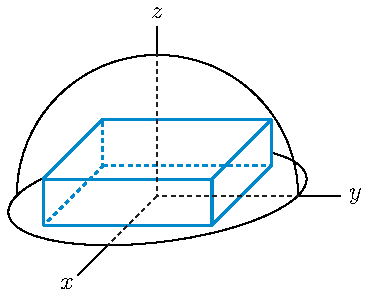
\includegraphics{inscSpher.pdf}
\end{center}
\end{question}

%\begin{hint}
%\end{hint}

\begin{answer}
$2\sqrt{3} \times 4\times 24$
\end{answer}

\begin{solution}
The optimal box will have vertices $(\pm x,\pm y, 0)$,
$(\pm x,\pm y,\ z)$ with $x,y,z>0$ and $z=48-4x^2-3y^2$. (If the lower
vertices are not in the $xy$--plane, the volume of the box can be increased
by lowering the bottom of the box to the $xy$--plane. If any of the four 
upper vertices are not on the hemisphere, the volume of the box can be 
increased by moving the upper vertices outwards to the hemisphere.)  
The volume of this box will be $(2x)(2y)z$. 
So we are to find the $x$, $y$ and $z$ that maximize the volume
$f(x,y,z)=4xyz$ subject to the constraint that 
$g(x,y,z)=48-4x^2-3y^2-z =0$. By the method of
Lagrange multipliers (Theorem~\eref{CLP200}{thm Lagrange} in the CLP-3 text),
the minimizing $x$, $y$, $z$ must obey
\begin{alignat*}{3}
f_x&=4yz=-8\la x&&=\la g_x\cr
f_y&=4xz=-6\la y&&=\la g_y\cr
f_z&=4xy=-\la&&=\la g_z\cr
&\hskip-0.2in 48-4x^2-3y^2-z&&=0
\end{alignat*}
Multiplying the first equation by $x$, the second equation by $y$ 
and the third equation by $z$  gives
\begin{align*}
4xyz&=-8\la x^2 \\
4xyz&=-6\la y^2 \\
4xyz&=-\la z
\end{align*}
This forces $8\la x^2=6\la y^2=\la z$. Since $\la$ cannot be zero (because
that would force $4xyz=0$), this in turn gives $8 x^2=6 y^2= z$. Substituting
in to the fourth equation gives
\begin{equation*}
48 -\frac{z}{2}-\frac{z}{2}-z=0\implies 2z=48\implies z=24,\ 8x^2=24,\
6y^2=24
\end{equation*}
The dimensions of the box of biggest volume are 
$2x=2\sqrt{3}$ by $2y=4$ by $z=24$.
\end{solution}

%%%%%%%%%%%%%%%%%%%%%%%%%%%%%%%%
\begin{question}[M200 2001D] %5
A rectangular bin is to be made of a wooden base and
heavy cardboard with no top. If wood is three times more expensive than
cardboard, find the dimensions of the cheapest bin which has a volume
of $12{\rm m}^3$.
\end{question}

%\begin{hint}
%
%\end{hint}

\begin{answer}
$2{\rm m}\times 2{\rm m}\times 3{\rm m}$
\end{answer}

\begin{solution}
Use units of money for which cardboard costs one unit per
square meter. Then, if the bin has dimensions $x\times y\times z$, it costs
$3xy+2xz+2yz$. We are to find the $x$, $y$ and $z$ that minimize the cost $f(x,y,z)=3xy+2xz+2yz$ subject to the constraint that $g(x,y,z)=xyz-12=0$. 
By the method of Lagrange multipliers (Theorem~\eref{CLP200}{thm Lagrange} 
in the CLP-3 text), the minimizing $x$, $y$, $z$ must obey
\begin{alignat*}{3}
f_x&=3y+2z&&=\la yz=\la g_x \\
f_y&=3x+2z&&=\la xz=\la g_y \\
f_z&=2x+2y&&=\la xy=\la g_z \\
&\ \ \ xyz-12&&=0
\end{alignat*}
Multiplying the first equation by $x$, the second equation by $y$ 
and the third equation by $z$ and then substituting in $xyz=12$ gives
\begin{align*}
3xy+2xz&=12\la \\
3xy+2yz&=12\la \\
2xz+2yz&=12\la 
\end{align*}
Subtracting the second equation from the first gives $2z(x-y)=0$.
Since $z=0$ is impossible, we must have $x=y$. Substituting this in
\begin{equation*}
3x^2+2xz=12\la\qquad 4xz=12\la
\end{equation*}
Subtracting
\begin{align*}
3x^2-2xz=0\implies z=\frac{3}{2}x
&\implies 12=xyz=\frac{3}{2}x^3
\implies x^3=8 \\
&\implies x=y=2,\ z=3\ {\rm meters}
\end{align*}
\end{solution}

%%%%%%%%%%%%%%%%%%%%%%%%%%%%%%%%
\begin{question}[M200 2000D] %5
A closed rectangular box having a volume of $4$ cubic metres
is to be built with material that costs \$8 per square metre for the sides
but \$12 per square metre for the top and bottom. Find the least expensive
dimensions for the box.
\end{question}

%\begin{hint}
%
%\end{hint}

\begin{answer}
$\frac{2}{\root 3\of 3}{\rm m}\times\frac{2}{\root 3\of 3}{\rm m}
                                \times 3^{2/3}{\rm m}$
\end{answer}

\begin{solution}
If the box has dimensions $x\times y\times z$, it costs
$24xy+16xz+16yz$. We are to find the $x$, $y$ and $z$ that minimize the cost $f(x,y,z)=24xy+16xz+16yz$ subject to the constraint that $g(x,y,z)=xyz-4=0$. 
By the method of Lagrange multipliers (Theorem~\eref{CLP200}{thm Lagrange} 
in the CLP-3 text), the minimizing $x$, $y$, $z$ must obey
\begin{alignat*}{3}
f_x&=24y+16z&&=\la yz=\la g_x \\
f_y&=24x+16z&&=\la xz=\la g_y \\
f_z&=16x+16y&&=\la xy=\la g_z \\
&\ \ \ \ \ \  xyz-4&&=0
\end{alignat*}
Multiplying the first equation by $x$, the second equation by $y$ 
and the third equation by $z$ and then substituting in $xyz=4$ gives
\begin{align*}
24xy+16xz&=4\la \\
24xy+16yz&=4\la \\
16xz+16yz&=4\la
\end{align*}
Subtracting the second equation from the first gives $16z(x-y)=0$.
Since $z=0$ is impossible, we must have $x=y$. Subbing this in
\begin{equation*}
24x^2+16xz=4\la\qquad 32xz=4\la
\end{equation*}
Subtracting
\begin{align*}
24x^2-16xz=0&\implies z=\frac{3}{2}x
\implies 4=xyz=\frac{3}{2}x^3
\implies x^3=\frac{8}{3} \\
&\implies x=y=\frac{2}{\root 3\of 3},\ z=3^{2/3}{\rm metres}
\end{align*}
\end{solution}

%%%%%%%%%%%%%%%%%%%%%%%%%%%%%%%%
\begin{question}[M200 2000A] %6
Suppose that $a$, $b$, $c$ are all greater than zero and let 
$D$ be the pyramid bounded by the plane $ax+by+cz=1$ and the 3 
coordinate planes. Use the method of Lagrange multipliers to find the 
largest possible volume of $D$ if the plane $ax + by + cz = 1$ is required 
to pass through the point $(1, 2, 3)$. (The volume of a pyramid is equal to one-third of the area of its base times the height.) 
\end{question}

%\begin{hint}
%
%\end{hint}

\begin{answer}
$a=\frac{1}{3}$, $b=\frac{1}{6}$, $c=\frac{1}{9}$,
max volume$ = 27$
\end{answer}

\begin{solution}
The vertices of the pyramid are $(0,0,0)$, 
$\big(\frac{1}{a},0,0\big)$, $\big(0, \frac{1}{b},0\big)$ and
$\big(0,0,\frac{1}{c}\big)$. So the base of the pyramid is a triangle
of area $\half\frac{1}{a}\frac{1}{b}$ and the height of the pyramid is
$\frac{1}{c}$. So the volume of the pyramid is $\frac{1}{6abc}$.
The plane passes through $(1,2,3)$ if and only if $a+2b+3c=1$. 
Thus we are to find the $a$, $b$ and $c$ that maximize the volume 
$f(a,b,c)=\frac{1}{6abc}$ subject to the constraint that 
$g(a,b,c)=a+2b+3c-1=0$. 
By the method of Lagrange multipliers (Theorem~\eref{CLP200}{thm Lagrange} 
in the CLP-3 text), the maximizing $a$, $b$, $c$ must obey
\begin{alignat*}{5}
f_a&=-\frac{1}{6a^2bc}&&=\la&=\la g_a\quad &&\iff\quad 6\la a^2bc&=-1 \\
f_b&=-\frac{1}{6ab^2c}&&=2\la&=\la g_b\quad&&\iff\quad 6\la ab^2c&=-\half \\
f_c&=-\frac{1}{6abc^2}&&=3\la&=\la g_c\quad      &&\iff\quad 
                                     6\la abc^2&=-\frac{1}{3}\\
    &a+2b+3c&&=1
\end{alignat*}
Dividing the first two equations gives $\frac{a}{b}=2$
and dividing the first equation by the third gives $\frac{a}{c}=3$.
Substituting $b=\half a$ and $c=\frac{1}{3} a$ in to the final equation gives
\begin{equation*}
a+2b+3c=3a=1  %\implies a=\frac{1}{3}
\implies a=\frac{1}{3},\ b=\frac{1}{6},\ c=\frac{1}{9}
\end{equation*}
and the maximum volume is $\frac{3\times 6\times 9}{6}=27$.
\end{solution}

%%%%%%%%%%%%%%%%%%
\subsection*{\Application}
%%%%%%%%%%%%%%%%%%

%%%%%%%%%%%%%%%%%%%%%%%%%%%%%%%%
\begin{question}[M200 2009D] %4
Use Lagrange multipliers to find the minimum distance from the origin 
to all points on the intersection of the curves
\begin{align*}
            g(x,y,z) &= x-z-4=0 \\
\text{and } h(x,y,z) &= x+y+z-3=0
\end{align*}
\end{question}

%\begin{hint}
%
%\end{hint}

\begin{answer}
$\sqrt{11}$
\end{answer}

\begin{solution}
We'll find the minimum distance$^2$ and then take the square root.
That is, we'll find the minimum of $f(x,y,z)=x^2+y^2+z^2$ subject to 
the constraints 
$g(x,y,z)=x-z-4=0$ and $h(x,y,z) = x + y + z -3=0$.
By Theorem \eref{CLP200}{thm doubleLagrange} in the CLP-3 text, 
any local minimum or maximum $(x,y,z)$ must obey the  double Lagrange 
multiplier equations
\begin{align*}
f_x = 2x &=\la + \mu  = \la g_x +\mu h_x\tag{E1} \\ 
f_y = 2y &= \mu = \la g_y +\mu h_y\tag{E2} \\ 
f_z = 2z &=-\la + \mu  = \la g_z +\mu h_z\tag{E3} \\ 
x - z &= 4\tag{E4} \\
x + y + z &= 3 \tag{E5}
\end{align*}
for some real numbers $\la$ and $\mu$. 
Adding (E1)and (E3) and then subtracting 2 times (E2) gives
\begin{equation*}
2x-4y+2z=0\qquad\text{or}\qquad
x-2y+z=0
\tag{E6}\end{equation*}
Substituting $x=4+z$ (from (E4)) into (E5) and (E6) gives
\begin{align*}
y+2z&=-1   \tag{E5'}\\
-2y+2z&=-4 \tag{E6'}
\end{align*}
Substituing $y=-1-2z$ (from (E5')) into (E6') gives
\begin{align*}
 6z =-6
\implies z=-1
\implies y=-1-2(-1)=1 
\implies x=4+(-1)=3
\end{align*}
So the closest point is $(3,1,-1)$ and the minimum
distance is $\sqrt{3^2+1^2+(-1)^2}=\sqrt{11}$.
\end{solution}

\begin{question}[M200 2014A] %4
Find the largest and smallest values of
\begin{equation*}
f(x,y,z) = 6x + y^2 + xz
\end{equation*}
on the sphere $x^2 + y^2 + z^2 = 36$. Determine all points at which 
these values occur.
\end{question}

%\begin{hint}
%
%\end{hint}

\begin{answer}
The min is $-12\sqrt{3}$ at $(-3\sqrt{3},0,3)$
and the max is $48$ at $(4,\pm 4,2)$.
\end{answer}

\begin{solution}
\emph{Solution 1:}\ \ \ 
This is a constrained optimization problem with objective function
$f(x,y,z) = 6 x +y^2 +xz$ and constraint function $g(x,y,z) =x^2+y^2+z^2-36$.
By Theorem \eref{CLP200}{thm Lagrange} in the CLP-3 text, any local minimum
or maximum $(x,y,z)$ must obey the  Lagrange multiplier equations
\begin{align*}
f_x = 6+z &=2 \la x = \la g_x \tag{E1} \\ 
f_y = 2y &=2 \la y = \la g_y \tag{E2} \\ 
f_z = x &=2 \la z = \la g_z \tag{E3} \\ 
x^2 + y^2 + z^2 &= 36 \tag{E4}
\end{align*}
for some real number $\la$. By equation (E2), $y(1-\la)=0$, which is
obeyed if and only if at least one of $y=0$, $\la=1$ is obeyed.
\begin{itemize}
\item 
If $y=0$, the remaining equations reduce to
\begin{align*}
6+z &=2 \la x  \tag{E1} \\ 
x &=2 \la z \tag{E3} \\ 
x^2  + z^2 &= 36 \tag{E4}
\end{align*}
Substituting (E3) into (E1) gives $6 + z = 4\la^ 2 z$, 
which forces $4\la^2\ne 1$ (since $6\ne 0$)
and gives $z = \frac{6}{4\la^2-1}$ and then 
$x=\frac{12\la}{4\la^2-1}$. Substituting this into (E4) gives
\begin{align*}
\frac{144\la^2}{{(4\la^2-1)}^2} +\frac{36}{{(4\la^2-1)}^2}&=36 \\
\frac{4\la^2}{{(4\la^2-1)}^2} +\frac{1}{{(4\la^2-1)}^2}&=1 \\
4\la^2+1 &= {(4\la^2-1)}^2 
\end{align*}
Write $\mu=4\la^2$. Then this last equation is
\begin{align*}
\mu+1 = \mu^2 -2\mu +1
&\iff \mu^2-3\mu =0 \\
&\iff \mu=0,3
\end{align*}
When $\mu=0$, we have $z=\frac{6}{\mu-1}=-6$ and $x=0$ (by (E4)).
When $\mu=3$, we have $z=\frac{6}{\mu-1}=3$ and then $x=\pm \sqrt{27}
=\pm 3\sqrt{3}$ (by (E4)).

\item
If $\la=1$, the remaining equations reduce to
\begin{align*}
6+z &=2 x  \tag{E1} \\ 
x &=2 z \tag{E3} \\ 
x^2  +y^2 + z^2 &= 36 \tag{E4}
\end{align*}
Substituting (E3) into (E1) gives $6+z=4z$ and hence $z=2$. Then (E3)
gives $x=4$ and (E4) gives $4^2 + y^2 + 2^2 =36$ or $y^2=16$ or $y=\pm 4$.
\end{itemize}
So we have the following candidates for the locations of the min and max
\begin{center}
\renewcommand{\arraystretch}{1.3}
     \begin{tabular}{|c|c|c|c|c|c|}
     \hline
       point
       &$(0,0, -6)$
       &$(3\sqrt{3},0,3)$
       &$(-3\sqrt{3},0,3)$
       &$(4,4,2) $
       &$(4,-4,2) $ \\ \hline
       value of $f$
       &$0$
       &$27\sqrt{3}$
       &$-27\sqrt{3}$
       &$48$ 
       &$48$\\ \hline
       &
       & 
       &min 
       &max
       &max \\ \hline
     \end{tabular}
\renewcommand{\arraystretch}{1.0}
\end{center}


\emph{Solution 2:}\ \ \ 
On the sphere we have $y^2=36-x^2-z^2$ and hence
$f= 36 + 6x +xz -x^2-z^2$ and $x^2+z^2\le 36$. So it suffices
to find the max and min of $h(x,z)= 36 + 6x +xz -x^2-z^2$
on the disk $D=\Set{(x,z)}{x^2+z^2\le 36}$. 
\begin{itemize}
\item
If a max or min occurs at an interior point $(x,z)$ of $D$,
then $(x,z)$ must be a critical point of $h$ and hence must obey
\begin{align*}
h_x = 6+z-2x&=0 \\
h_z = x-2z=0
\end{align*}
Substituting $x=2z$ into the first equation gives $6-3z=0$ 
and hence $z=2$ and $x=4$.

\item
If a max or min occurs a point $(x,z)$ on the boundary of $D$, we 
have  $x^2+z^2=36$ and hence $x=\pm\sqrt{36-z^2}$ and $h=6x+zx=\pm(6+z)\sqrt{36-z^2}$ with 
$-6\le z\le 6$. So the max or min can occur either when $z=-6$ or $z=+6$
or at a $z$ obeying
\begin{align*}
0=\diff{}{z}\big[(6+z)\sqrt{36-z^2}\big]
 =\sqrt{36-z^2} - \frac{z(6+z)}{\sqrt{36-z^2}}
\end{align*}
or equivalently
\begin{align*}
36-z^2-z(6+z)&=0 \\
2z^2 +6z -36 &=0 \\
z^2 +3z -18 &=0 \\
(z+6)(z-3)&=0
\end{align*}
So the max or min can occur either when $z=\pm 6$ or $z=3$.
\end{itemize}
So we have the following candidates for the locations of the min and max
\begin{center}
\renewcommand{\arraystretch}{1.3}
     \begin{tabular}{|c|c|c|c|c|c|}
     \hline
       point
       &$(0,0, \pm 6)$
       &$(3\sqrt{3},0,3)$
       &$(-3\sqrt{3},0,3)$
       &$(4,4,2) $
       &$(4,-4,2) $ \\ \hline
       value of $f$
       &$0$
       &$27\sqrt{3}$
       &$-27\sqrt{3}$
       &$48$ 
       &$48$\\ \hline
       &
       & 
       &min 
       &max
       &max \\ \hline
     \end{tabular}
\renewcommand{\arraystretch}{1.0}
\end{center}
\end{solution}

%%%%%%%%%%%%%%%%%%%%%%%%%%%%%%%%
\begin{question}[M200 2016D] %5
\item %5 
The temperature in the plane is given by $T(x,y) = e^y\big(x^2+y^2\big)$.
\begin{enumerate}[(a)]
\item
\begin{enumerate}[(i)]
\item
Give the system of equations that must be solved in order to find the 
warmest and coolest point on the circle $x^2+y^2=100$ by the method
of Lagrange multipliers.
\item 
Find the warmest and coolest points on the circle by solving that system.
\end{enumerate}

\item 
\begin{enumerate}[(i)]
\item
Give the system of equations that must be solved in order to find the
critical points of $T(x,y)$.
\item
Find the critical points by solving that system.
\end{enumerate}

\item
Find the coolest point on the solid disc $x^2+y^2\le 100$.

\end{enumerate}
\end{question}

%\begin{hint}
%
%\end{hint}

\begin{answer}
(a) (i)
\begin{align*}
 2x\,e^y &=\la (2x) \\
e^y\big(x^2+y^2+2y\big) &=\la (2y) \\
x^2+y^2&=100 
\end{align*}

(a) (ii)  The warmest point is $(0,10)$ and the coolest point is $(0,-10)$.

(b) (i)
\begin{align*}
2x\,e^y &=0 \\
e^y\big(x^2+y^2+2y\big) &=0  
\end{align*} 
(b) (ii) $(0,0)$ and $(0,-2)$

(c) $(0,0)$
\end{answer}

\begin{solution}
By way of preparation, we have
\begin{align*}
\pdiff{T}{x}(x,y) =  2x\,e^y\qquad
\pdiff{T}{y}(x,y) =  e^y\big(x^2+y^2+2y\big)
\end{align*}

(a) (i) 
For this problem the objective function is $T(x,y) = e^y\big(x^2+y^2\big)$
and the constraint function is $g(x,y)=x^2 + y^2 - 100$. 
According to the method of Lagrange multipliers, Theorem \eref{CLP200}{thm Lagrange}
in the CLP-3 text, we need to find all solutions to
\begin{align*}
T_x = 2x\,e^y &=\la (2x) = \la g_x \tag{E1}\\
T_y = e^y\big(x^2+y^2+2y\big) &=\la (2y) = \la g_y \tag{E2}\\
x^2+y^2&=100 \tag{E3}
\end{align*}

(a) (ii)
According to equation (E1), $2x(e^y-\la)=0$. This condition is satisfied
if and only if at least one of $x=0$, $\la=e^y$ is obeyed.
\begin{itemize}
\item 
If $x=0$, then equation (E3) reduces to $y^2=100$, which is obeyed if $y=\pm 10$.
Equation (E2) then gives the corresponding values for $\la$, which we don't need.

\item
If $\la=e^y$, then equation (E2) reduces to
\begin{equation*}
e^y\big(x^2+y^2+2y\big) = (2y)e^y
\iff 
e^y\big(x^2+y^2\big)=0
\end{equation*}
which conflicts with (E3). So we can't have $\la=e^y$.
\end{itemize}
So the only possible locations of the maximum and minimum of the function
$T$ are $(0,10)$ and $(0,-10)$. To complete the problem, we only have to 
compute $T$ at those points.
\begin{center}
\renewcommand{\arraystretch}{1.3}
     \begin{tabular}{|c|c|c|}
     \hline
       point
       &$(0,10)$
       &$(0,-10)$ \\ \hline
       value of $T$
       &$100 e^{10}$
       &$100 e^{-10}$ \\ \hline
       &max 
       &min  \\ \hline
     \end{tabular}
\renewcommand{\arraystretch}{1.0}
\end{center}
Hence the maximum value of $T(x,y) = e^y\big(x^2+y^2\big)$ on $x^2 + y^2 = 100$ 
is $100 e^{10}$ at $(0,10)$ and the minimum value is $100 e^{-10}$ at $(0,-10)$.

We remark that, on $x^2+y^2=100$, the objective function 
$T(x,y) = e^y\big(x^2+y^2\big) = 100 e^y$. So of course the maximum value of
$T$ is achieved when $y$ is a maximum, i.e. when $y=10$, 
and the minimum value of
$T$ is achieved when $y$ is a minimum, i.e. when $y=-10$.

(b) (i) By definition, the point $(x,y)$ is a critical point of $T(x,y)$ if ane only if
\begin{align*}
T_x = 2x\,e^y &=0 \tag{E1}\\
T_y = e^y\big(x^2+y^2+2y\big) &=0  \tag{E2}
\end{align*}

(b) (ii) 
Equation (E1) forces $x=0$. When $x=0$, equation (E2) reduces to
\begin{align*}
e^y\big(y^2+2y\big) =0 
\iff  y(y+2)=0
\iff y=0\text{ or }y=-2
\end{align*}
So there are two critical points, namely $(0,0)$ and $(0,-2)$.

(c) 
Note that $T(x,y) = e^y\big(x^2+y^2\big)\ge 0$ on all of $\bbbr^2$.
As $T(x,y)=0$ only at $(0,0)$, it is obvious that $(0,0)$ is the coolest point.


In case you didn't notice that, here is a more conventional solution.

The coolest point on the solid disc $x^2+y^2\le 100$
must either be on the boundary, $x^2+y^2= 100$, of the disc
or be in the interior, $x^2+y^2 < 100$, of the disc.
 
In part (a) (ii) we found that the coolest point on the boundary 
is $(0,-10)$, where $T=100 e^{-10}$. 


If the coolest point is in the interior, it must be a critical point and so must be 
either $(0,0)$, where $T=0$, or $(0,-2)$, where $T= 4e^{-2}$.

So the coolest point is $(0,0)$.
\end{solution}



%%%%%%%%%%%%%%%%%%%%%%%%%%%%%%%%%%%%%%%%%
\begin{question} [M200 2002D] % 5
\begin{enumerate}[(a)]
\item 
By finding the points of tangency, determine the values of $c$ for 
which $x+y+z=c$ is a tangent plane to the surface $4x^2+4y^2+z^2=96$.
\item
Use the method of Lagrange Multipliers to determine the absolute
maximum and minimum values of the function $f(x,y,z)=x+y+z$ along the surface
$g(x,y,z)=4x^2+4y^2+z^2=96$.
\item
Why do you get the same answers in (a) and (b)?
\end{enumerate}
\end{question}

%\begin{hint}
%
%\end{hint}

\begin{answer}
(a) $c=\pm 12$ \qquad
(b) $\pm 12$

(c) The level surfaces of $x+y+z$ are planes with equation of the
form $x+y+z=c$. To find the largest (smallest) value of 
$x+y+z$ on $4x^2+4y^2+z^2=96$ we keep increasing (decreasing) $c$ until
we get to the largest (smallest) value of $c$ for which the plane 
$x+y+z=c$ intersects $4x^2+4y^2+z^2=96$. For this value of $c$, 
$x+y+z=c$ is tangent to $4x^2+4y^2+z^2=96$.
\end{answer}

\begin{solution}
(a) A normal vector to $F(x,y,z)=4x^2+4y^2+z^2=96$ at 
$(x_0,y_0,z_0)$ is $\vnabla F(x_0,y_0,z_0)=\llt 8x_0,8y_0,2z_0\rgt$. 
(Note that this normal vector is never the zero vector because $(0,0,0)$
is not on the surface.) So the tangent plane
to $4x^2+4y^2+z^2=96$ at $(x_0,y_0,z_0)$ is
\begin{equation*}
8x_0(x-x_0)+8y_0(y-y_0)+2z_0(z-z_0)=0\quad\text{or}\quad
8x_0x+8y_0y+2z_0z=8x_0^2+8y_0^2+2z_0^2
\end{equation*}
This plane is of the form $x+y+z=c$ if and only if $8x_0=8y_0=2z_0$.
A point $(x_0,y_0,z_0)$ with $8x_0=8y_0=2z_0$ is on the surface 
$4x^2+4y^2+z^2=96$ if and only if
\begin{equation*}
4x_0^2+4y_0^2+z_0^2=4x_0^2+4x_0^2+(4x_0)^2=96
\iff 24 x_0^2=96
\iff x_0^2=4
\iff x_0=\pm 2
\end{equation*}
When $x_0=\pm 2$, we have $y_0=\pm 2$ and $z_0=\pm 8$ (upper signs go together
and lower signs go together) so that the tangent plane $8x_0x+8y_0y+2z_0z=8x_0^2+8y_0^2+2z_0^2$
is
\begin{align*}
8(\pm 2)x+8(\pm 2)y+2(\pm 8)z=8(\pm 2)^2+8(\pm 2)^2+2(\pm 8)^2
&\quad\text{or}\quad
\pm x \pm y \pm z=2+2+8\\
&\quad\text{or}\quad
 x + y + z=\mp 12\\
&\implies  c=\pm 12
\end{align*}

(b)
We are to find the $x$, $y$ and $z$ that minimize or maximize 
$f(x,y,z)=x+y+z$ subject to the constraint that 
$g(x,y,z)=4x^2+4y^2+z^2-96=0$. By the method of
Lagrange multipliers (Theorem~\eref{CLP200}{thm Lagrange} in the CLP-3 text),
the minimizing/maximizing $x$, $y$, $z$ must obey
\begin{alignat*}{3}
f_x&=1=\la(8x)&&=\la g_x\\
f_y&=1=\la(8y)&&=\la g_y\\
f_z&=1=\la(2z)&&=\la g_z\\
&\hskip-0.6in 4x^2+4y^2+z^2-96&&=0
\end{alignat*}
The first three equations give 
\begin{equation*}
x=\frac{1}{8\la}\qquad y=\frac{1}{8\la}\qquad z=\frac{1}{2\la}
\qquad\text{with }\la\ne 0
\end{equation*}
Substituting this into the fourth equation gives
\begin{align*}
4\left(\frac{1}{8\la}\right)^2+4\left(\frac{1}{8\la}\right)^2
+\left(\frac{1}{2\la}\right)^2=96 
&\iff
\left(\frac{1}{16}+\frac{1}{16}+\frac{1}{4}\right)\frac{1}{\la^2}=96 \\
&\iff
\la^2=\frac{3}{8}\frac{1}{96}=\frac{1}{8\times 32} \\
&\iff \la=\pm \frac{1}{16}
\end{align*}
Hence $x=\pm 2$, $y=\pm 2$ and $z=\pm 8$ so that the largest and smallest
values of $x+y+z$ on $4x^2+4y^2+z^2-96$ are $\pm 2\pm2 \pm 8$ or
$\pm 12$.

(c) The level surfaces of $x+y+z$ are planes with equation of the
form $x+y+z=c$. To find the largest (smallest) value of 
$x+y+z$ on $4x^2+4y^2+z^2=96$ we keep increasing (decreasing) $c$ until
we get to the largest (smallest) value of $c$ for which the plane 
$x+y+z=c$ intersects $4x^2+4y^2+z^2=96$. For this value of $c$, 
$x+y+z=c$ is tangent to $4x^2+4y^2+z^2=96$.
\end{solution}

%%%%%%%%%%%%%%%%%%%%%%%%%%%%%%%%
\begin{question}
Let $f(x,y)$ have continuous partial derivatives. Consider the problem of 
finding local minima and maxima of $f(x,y)$ on the curve $xy=1$.
\begin{itemize}
\item
Define $g(x,y) = xy -1$.
According to the method of Lagrange multipliers, if $(x,y)$ is 
a local minimum or maximum of $f(x,y)$ on the curve $xy=1$, then there is a real number $\la$ such that
\begin{equation*}
\vnabla f(x,y) =\la \vnabla g(x,y),\quad g(x,y)=0
\tag{E1}\end{equation*}

\item
On the curve $xy=1$, we have 
$y=\frac{1}{x}$ and $f(x,y) =f\big(x,\frac{1}{x}\big)$. Define 
$F(x)=f\big(x,\frac{1}{x}\big)$. If $x\ne 0$ is a local minimum or maximum of 
$F(x)$, we have that
\begin{equation*}
F'(x)=0
\tag{E2}\end{equation*}
\end{itemize}
Show that (E1) is equivalent to (E2), in the sense that 
\begin{align*}
&\text{there is a $\la$ such that $(x,y,\la)$  obeys (E1)}\\
&\hskip-0.5in\text{if and only if}\\ 
&\text{$x\ne 0$ obeys (E2) and $y=\nicefrac{1}{x}$.}
\end{align*}
\end{question}

%\begin{hint}
%
%\end{hint}

\begin{answer}
See the solution.
\end{answer}

\begin{solution}
Note that if $(x,y)$ obeys $g(x,y)=xy-1=0$, then $x$ is necessarily nonzero.
So we may assume that $x\ne 0$. Then
\begin{align*}
&\text{There is a $\la$ such that $(x,y,\la)$ obeys (E1)} \\
&\hskip0.2in
  \iff \text{there is a $\la$ such that }
        f_x(x,y)=\la g_x(x,y),\quad f_y(x,y)=\la g_y(x,y),\quad g(x,y)=0 \\
&\hskip0.2in
  \iff \text{there is a $\la$ such that }
           f_x(x,y)=\la y,\quad f_y(x,y)=\la x,\quad xy=1 \\
&\hskip0.2in
  \iff \text{there is a $\la$ such that }
      \frac{1}{y}f_x(x,y)= \frac{1}{x} f_y(x,y)=\la ,\quad xy=1 \\
&\hskip0.2in
  \iff  \frac{1}{y}f_x(x,y)= \frac{1}{x} f_y(x,y) ,\quad xy=1 \\
&\hskip0.2in
  \iff  xf_x\Big(\!x,\frac{1}{x}\Big)= \frac{1}{x} 
        f_y\Big(\!x,\frac{1}{x}\Big) ,\quad y=\frac{1}{x} \\
&\hskip0.2in
  \iff F'(x) = \diff{}{x} f\Big(\!x,\frac{1}{x}\Big) 
             = f_x\Big(\!x,\frac{1}{x}\Big)
              -\frac{1}{x^2}f_y\Big(\!x,\frac{1}{x}\Big)
             =0,\quad y=\frac{1}{x}
\end{align*}


\end{solution}


